The optimization of the Electric Vehicle Charging Station (EVCS) network is addressed through a multi-objective optimization approach considering five conflicting objectives: maximizing charger speed, maximizing coverage, minimizing the number of stations, minimizing the number of chargers, and minimizing the average distance between EVCS and electric vehicles (EVs). This work employs the \textbf{NSGA-II (Non-dominated Sorting Genetic Algorithm II)} to solve this problem \cite{A_Fast_and_Elitist_Multi_objective_Genetic_Algorithm_NSGA_II}. The methodology is divided into two primary parts:  
\textbf{(A)} finding a single optimized solution, and  
\textbf{(B)} finding the Pareto front representing the set of optimal trade-off solutions.

\subsection*{NSGA-II for EVCS Networks: Project Approach}

The project applies NSGA-II systematically to optimize the EVCS network by addressing two main tasks: identifying a single optimized solution and discovering the Pareto front of optimal solutions that balance the competing objectives \cite{Introduction_to_evolutionary_computing}.

\subsubsection*{Problem Formulation}

The EVCS network optimization requires balancing several competing objectives:

\begin{itemize}
    \item \textbf{Maximize Charger Speed (Upgrade to Level 3):} Upgrade all chargers to Level 3, providing at least 50 kW power output, to reduce waiting times and improve efficiency.
    \item \textbf{Maximize Coverage:} Ensure the selected stations cover the largest geographic area possible.
    \item \textbf{Minimize Number of Stations:} Reduce infrastructure cost by minimizing the number of stations deployed.
    \item \textbf{Minimize Number of Chargers:} Avoid overcapacity and excess cost by optimizing charger count.
    \item \textbf{Minimize Average Distance:} Reduce travel distance for EV users to reach the nearest charging station.
\end{itemize}

These five objectives create a complex trade-off problem, where improving one objective might negatively affect another. NSGA-II tackles this by generating a set of optimal solutions instead of a single answer \cite{A_Fast_and_Elitist_Multi_objective_Genetic_Algorithm_NSGA_II}.

\bigskip
\textbf{Part A: Finding a Single Optimized Solution}

This part focuses on identifying one optimized configuration of EVCS stations that balances the five objectives.

\paragraph{1. Representation of Solutions (Chromosomes)}  
Each individual solution in the population is encoded as a chromosome, representing the selection and characteristics (e.g., number of chargers, charger speed) of candidate stations \cite{Introduction_to_evolutionary_computing}.

\paragraph{2. Fitness Evaluation}  
Each solution’s fitness is evaluated based on the five objectives:

\begin{enumerate}
    \item \textbf{Maximize Charger Speed:} Chargers have power levels \( P_i \in \{11.5,\, 14.2,\, 19.2,\, 25,\, 60,\, 62,\, 80,\, 120,\, 150,\, 180,\, 200,\, 240,\, 250,\, 300,\, 325,\, 350,\, 400\} \) kW. The focus is on upgrading to Level 3 chargers with power ratings of at least 50 kW.    
    \item \textbf{Maximize Coverage:} Calculate and maximize the geographic area covered by selected stations.
    \item \textbf{Minimize Number of Stations:} Penalize solutions using more stations than necessary.
    \item \textbf{Minimize Number of Chargers:} Penalize solutions with excessive chargers.
    \item \textbf{Minimize Average Distance:} Minimize average travel distance for EVs.
\end{enumerate}

These objectives combine into a fitness function measuring overall solution quality \cite{Introduction_to_evolutionary_computing}.

\paragraph{3. Selection, Crossover, and Mutation}  
NSGA-II applies evolutionary operators:

\begin{itemize}
    \item \textbf{Selection:} Chooses individuals based on Pareto dominance ranking.
    \item \textbf{Crossover:} Combines two parent solutions to create offspring with mixed characteristics.
    \item \textbf{Mutation:} Introduces random changes to maintain diversity and avoid premature convergence.
\end{itemize}

\paragraph{Result of Part A}  
The outcome is a single viable solution balancing the five objectives, offering a practical EVCS network configuration.

\bigskip
\textbf{Part B: Finding the Pareto Front – Pareto-Optimal Solutions}

This part finds the \textbf{Pareto front}, a set of solutions where improving one objective worsens at least one other.

\paragraph{1. Non-Dominated Sorting}  
NSGA-II ranks solutions into fronts based on Pareto dominance:

\begin{itemize}
    \item \textit{Front 1:} Solutions not dominated by any other.
    \item \textit{Front 2:} Solutions dominated only by Front 1 members.
    \item And so on.
\end{itemize}

\paragraph{2. Crowding Distance Calculation}  
Calculates how isolated solutions are in objective space to maintain diversity by preferring individuals in less crowded regions.

\paragraph{Result of Part B}  
The \textbf{Pareto front} (Front 1) consists of the best trade-off solutions, offering various EVCS configurations optimized for different priorities \cite{A_Fast_and_Elitist_Multi_objective_Genetic_Algorithm_NSGA_II}.

\subsection*{Final Interpretation of Results}

\paragraph{A) Single Solution}  
The single solution provides a balanced and practical EVCS configuration that optimizes multiple objectives, though it may not be the best for all.

\paragraph{B) Pareto Front}  
The Pareto front offers a set of optimal solutions, giving decision-makers the flexibility to select configurations based on specific strategic goals like cost, coverage, or distance \cite{Introduction_to_evolutionary_computing}.

\paragraph{Summary}  
NSGA-II effectively generates a diverse set of Pareto-optimal solutions, enabling multi-objective optimization of EVCS networks and providing decision-makers with flexible deployment strategies balancing coverage, speed, cost, and accessibility \cite{A_Fast_and_Elitist_Multi_objective_Genetic_Algorithm_NSGA_II}.

\subsubsection*{NSGA-II Flowchart}

Figure~\ref{fig:evcs_nsga_flowchart} illustrates the NSGA-II algorithm workflow for EVCS network optimization:

\begin{enumerate}
    \item \textbf{Initialize Population:} Randomly generate initial solutions.
    \item \textbf{Evaluate Fitness:} Calculate all objectives for each solution.
    \item \textbf{Non-Dominated Sorting:} Rank solutions into Pareto fronts.
    \item \textbf{Crowding Distance Calculation:} Measure solution diversity.
    \item \textbf{Selection:} Choose individuals based on Pareto rank and crowding distance.
    \item \textbf{Crossover and Mutation:} Generate new offspring solutions.
    \item \textbf{Combine and Sort:} Merge parents and offspring; re-rank.
    \item \textbf{Next Generation:} Select the best individuals for the next generation.
    \item \textbf{Termination:} Repeat until max generations reached.
\end{enumerate}

This iterative process yields a Pareto front of non-dominated solutions representing optimal trade-offs.

\begin{figure}[h]
    \centering
    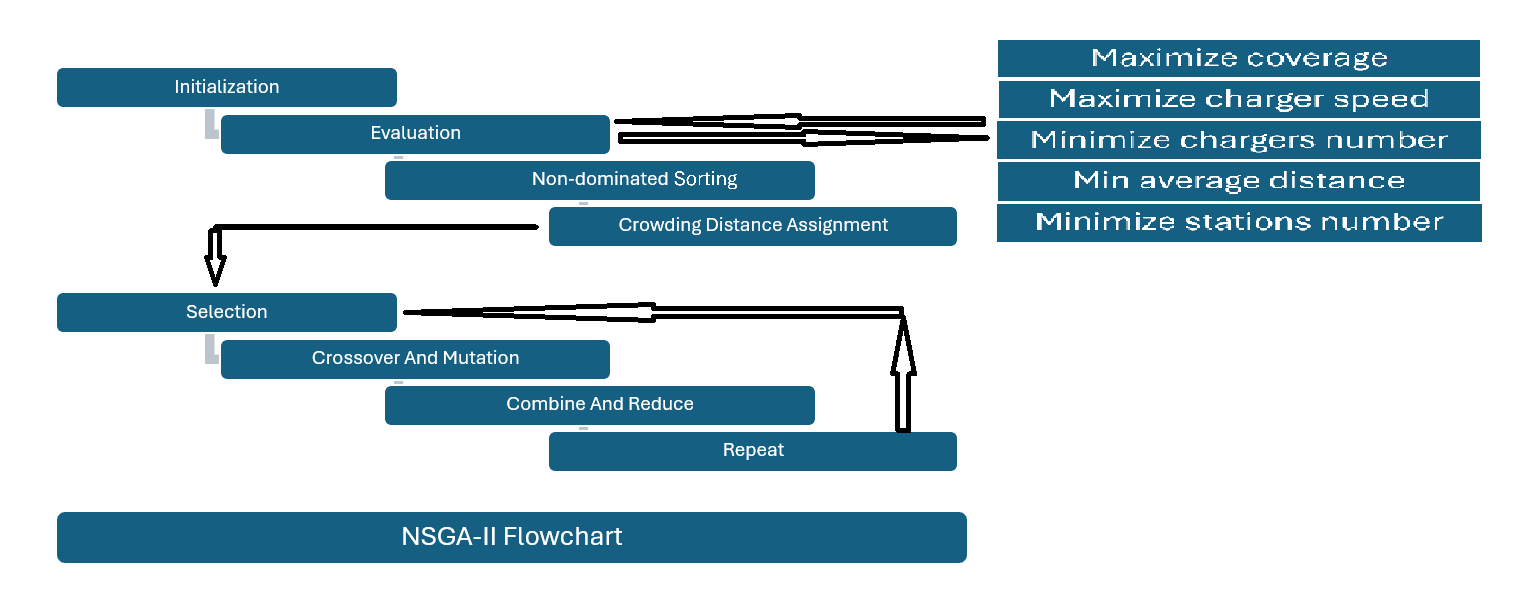
\includegraphics[width=0.8\textwidth]{..//Figures/evcs-nsga-flowchart.png}
    \caption{Flowchart of the NSGA-II algorithm for EVCS network optimization.}
    \label{fig:evcs_nsga_flowchart}
\end{figure}